% id: 63-e2
% book: 100발100중 3-2 중간 · 01 3-2 중간(삼각비·삼각비의 활용·원과 직선·원주각·부록)
% section: 서술형 문제
% figure: crop:fig-63-e2-2.png
% answer: $50^\circ$
% answer_source: 예제 모범답안
% variant_level: 0 (원본 전사)
% 이 파일은 build.mjs 가 items.json 에서 만든다. 고칠 때는 items.json 을 고친다.
\smash{\raisebox{1.5mm}{\dmkichul{100발100중 3-2 중간 63쪽 예제 2 · 예제}}}
\noindent\begin{minipage}[t]{0.58\linewidth}\vspace{0pt}\raggedright 그림에서 $\seg{OM}=\seg{ON}$이고 $\angle\pt{B}=65^\circ$일 때, $\angle\pt{BAC}$의 크기를 구하고, 그 과정을 서술하시오. \mbox{[5점]}\end{minipage}\hfill\begin{minipage}[t]{0.4\linewidth}\vspace{0pt}\centering 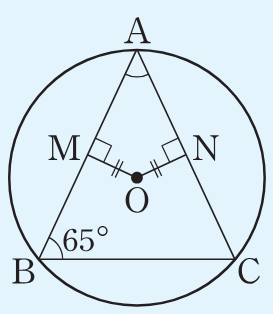
\includegraphics[width=65.3pt]{figures/fig-63-e2-2.png}\end{minipage}\par
